\chapter{Methodology}
To ensure the success of this project a basic plan of action was created. The following diagram shows the critical phases of the project, as interpreted from the terms of reference.

\begin{figure}[!ht] 
\captionsetup{width=0.8\linewidth, font=small}  
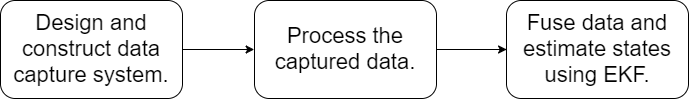
\includegraphics[width=0.8\linewidth]{figures/planOfAction.png}
\caption{Diagram showing the progression and dependence of the major stages of this project}
\label{fig:planOfAction}
\end{figure}

Due to the availability of equipment, financial limitations and time constraints various design parameters where predetermined. These known elements were central to the design process.
  
\section{System Design}
This section is dedicated to defining and understanding the specifications of the data capture system. Due to the lack of existing literature on wearable motion capture systems a starting point had to be determined. This point would serve as the first iteration of an iterative design process to fufill all defined requirements.

Work completed by Stocks \cite{bradstocks} was used as this starting point. The original system comprised of 2 GoPro Hero Session cameras rigidly connected to a Sony smartphone acting as the main sensor. This was all mounted to a GoPro Fetch harness \cite{fetch} such that it could be carried by various quadrupeds. The original system is pictured below.

\begin{figure}[!ht] 
\captionsetup{width=0.8\linewidth, font=small}  
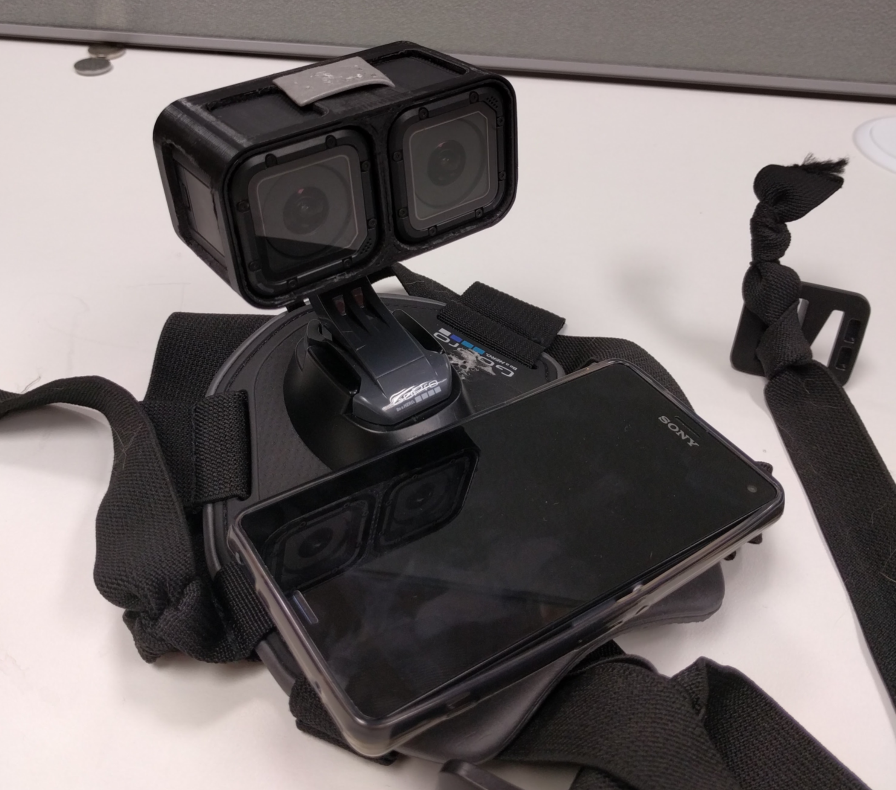
\includegraphics[width=0.8\linewidth]{figures/p1.png}
\caption{Original wearable motion capture system designed by Stocks, image from \cite{bradstocks}}
\label{fig:p1}
\end{figure}

The system was adapted to use 4 GoPro Hero Session cameras and an IMU mounted to the torso of the subject. Two of the four cameras mounted to the chest of the subject and the other two mounted to the middle-back of the subject. 

The cameras will record the lower limbs of the subject while the IMU will log inertial data from the body of the subject. By having cameras on both the chest and back of the subject, the front and rear elements of the gait can be captured. The video data from the cameras will provide information about the kinematics of the lower limbs with respect to the cameras while the IMU will provide motion data of the body with respect to the inertial frame. 

The following equipment was provided by the Mechatronics Research Lab and was chosen as the main components to use in the system

\begin{table}[!ht]
\label{equipment-table}
\begin{tabular}{llll}
Item		& Selected Equipment				& From	\\
Camera      & 4 GoPro Hero Session Cameras  & \cite{gopro}\\
IMU         & 1 Sony Xperia Z3 Compact      & \cite{sony}\\
Chest Mount & 1 Action Mount Chest Mount    & \cite{actionmounts}   
\end{tabular}
\caption{Known design elements of the project}
\end{table}


The problem space and concept design of the system has been outlined above, but to further the design process designable specifications need to be defined. By looking at the various limitations of existing systems and the available components the following specifications were identified.

\begin{itemize}
\item Two stereo housings to hold the cameras
\item Housing to hold the smartphone
\item Chest mount to hold the cameras and IMU
\item Connecting hardware to mount camera housing to the chest harness
\item Cameras must be stable during running
\item IMU must be rigidly mounted to front cameras
\item Cameras must capture full lower limb motion
\item Harness must be comfortable during running
\item Harness must not impede natural gait of subject
\item Harness must be as light as possible
\item Harness must fit different size torsos
\item Harness must be unisex
\item System must be remote controlled as far as possible 
\end{itemize}

These specifications ensure a system that can be used by a large demographic of people. This allows the system to be used in a variety of applications from engineering to medical science. The system can also be used by subjects with prosthesis as it requires only markers to be attached to the lower limbs. This is extremely usefull in the rehabilitation of amputee subjects.

\section{Modelling the Lower Limbs}
To interpret the data and the underlying mathematics a model of the human torso and lower limbs must be created. This model consist of the lower limbs being represented as rigid links. Each leg is comprised of three different links: a thigh, calf and foot. The joints connecting the links have limited degrees of freedom to simplify the model. The ankle (serving as the joint between the foot and calf) is assumed to have a single rotational degree of freedom (pitch). The knee (serving as a joint between the calf and the thigh) has also been limited to only have a pitch element. Finally the hip (joining the thigh to the body) has been given 2 rotational degrees of freedom: pitch and yaw. This rigid model can be seen in the following figure.

\begin{figure}[!ht] 
\captionsetup{width=0.8\linewidth, font=small}  
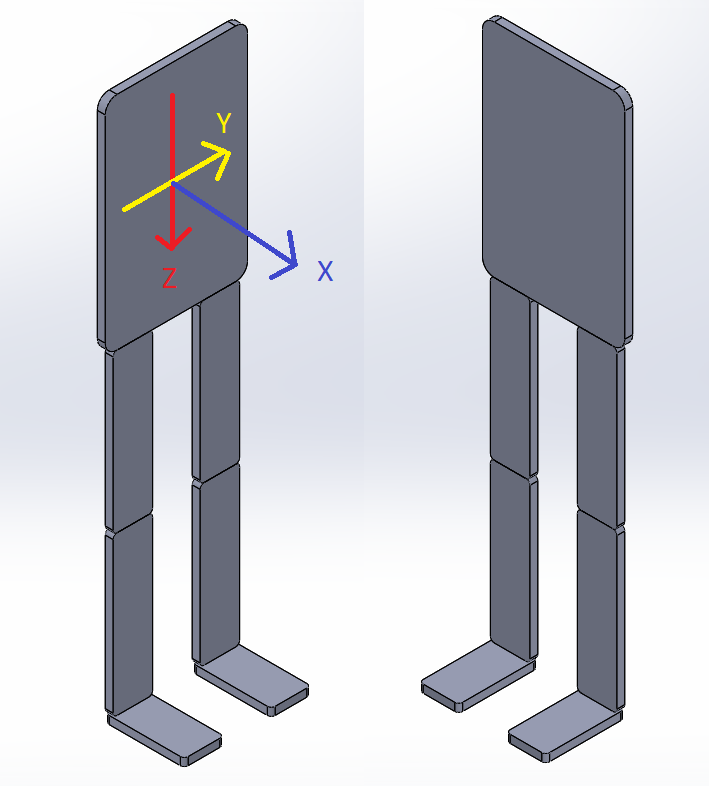
\includegraphics[width=0.8\linewidth]{figures/swmodel.png}
\caption{Rigid beam model used to model the lower limbs of a biped}
\label{fig:swmodel}
\end{figure}

A very important benefit to using such a model it the transferability to a robotic implementation of the lower limbs. Often robot joints are implemented using a variety of DC machines or servomotors. by limiting the freedom of various joints we simplify the joints and reduce the amount of servomotors required to mimic the model. This allows for both cheaper and less complex bipedal robotic limbs to be constructed.

\section{Experimental Details}
The data was captured during a short straight road run where the runner started from a standing position and accelerated to a steady state running pace. This allowed us to capture some transients (accelerations) from the run that can be used to initialize the proposed EKF. The run lasted about 18 seconds providing us with 1800 datapoints. The test was performed 3 times and a final dataset was chosen after examining the data gathered.

\section{Limitations}
The scope of this research does not include runs over rough terrain as this is the logical next step after flat ground steady state running is modelled and estimated correctly. It is assumed that given robust EKF and complete image processing solution the system would be transferable for running on various terrains.

This research will also not analyse the running style, efficiency or balance of the subjects, since this thesis concerned with the engineering involved in creating a novel data capture system. 

Another source of limitations is the nature of the rigid beam model. This non elastic model does not take in to account the slight compression and expansion of the limbs during running. The model also omits yaw and roll parameters about the knee and ankle as well as roll parameters about the hip; reducing the overall completeness of the model for the sake of simplicity. Finally the model assumes a rigid stationary chest that introduces some error relating the camera data.

In steady state running the chest will rotate opposite to the hips to balance the angular momentum of the runner. Since the chest swings at a rate proportional to the gait period this could be modelled as a harmonic oscillator. This idea was explored in \cite{patel2017trackingieee} where the cheetah spine was partly modelled in this fashion with positive results. It would also be possible to interpret the rotational rates of the chest from the IMU data.

Various limitations are inherent in this project due to its novelty. These limitations have been noted such that future work could improve upon certain elements while this foundational work serves as a point of reference.

 









 



















